% Portfolio de projets — Ismaila DEH
% Compilation : pdflatex portfolio.tex (depuis le dossier cv/)
\documentclass[11pt,a4paper]{article}
\usepackage[utf8]{inputenc}
\usepackage[T1]{fontenc}
\usepackage[french]{babel}
\usepackage{lmodern}
\usepackage[margin=2cm]{geometry}
\usepackage{graphicx}
\usepackage{xcolor}
\usepackage{booktabs}
\usepackage{tabularx}
\usepackage{amsmath}
\usepackage{titlesec}
\usepackage{enumitem}
\usepackage{fancyhdr}
\usepackage[hidelinks]{hyperref}

\definecolor{accent}{HTML}{1F4E79}
\definecolor{gris}{HTML}{6B675F}
\graphicspath{{../projets/}}

\titleformat{\section}{\Large\bfseries\color{accent}}{\thesection}{0.8em}{}[\vspace{-0.6em}\textcolor{accent}{\rule{\linewidth}{0.6pt}}]
\titlespacing*{\section}{0pt}{1.2em}{0.8em}
\setlist{nosep,leftmargin=1.4em}
\pagestyle{fancy}\fancyhf{}
\renewcommand{\headrulewidth}{0pt}
\fancyfoot[L]{\small\color{gris}Ismaila DEH · Portfolio de physique numérique}
\fancyfoot[R]{\small\color{gris}\thepage}

\newcommand{\chiffre}[2]{\begin{minipage}[t]{0.23\linewidth}\centering{\Huge\color{accent}#1}\\[2pt]{\footnotesize\color{gris}\MakeUppercase{#2}}\end{minipage}}
\newcommand{\lien}[1]{\noindent\href{https://github.com/IsmailaDEH/Ismaila/tree/main/projets/#1}{\small\color{accent}\texttt{github.com/IsmailaDEH/Ismaila/projets/#1}}}

\begin{document}

% ------------------------------------------------------------------ Page de garde
\thispagestyle{empty}
\vspace*{2cm}
{\color{gris}\small\texttt{ISMAILA DEH · ÉTUDIANT EN PHYSIQUE}}\\[0.6cm]
{\fontsize{38}{42}\selectfont\bfseries Physique numérique\\[4pt]\color{gris}\itshape \& modélisation}\\[1cm]
\begin{minipage}{0.85\linewidth}\large
Je construis des simulations de systèmes physiques (chaos, transitions de phase, diffusion, orbites) et je les confronte à la théorie. J'utilise aussi l'apprentissage automatique pour retrouver des lois physiques à partir de données.
\end{minipage}

\vspace{1.5cm}
\noindent\chiffre{5}{projets}\hfill\chiffre{0,9\,\%}{erreur sur $T_c$ (Ising)}\hfill\chiffre{0,13\,\%}{erreur Lorenz (SINDy)}\hfill\chiffre{19}{tests automatiques}

\vspace{1.5cm}
\begin{center}
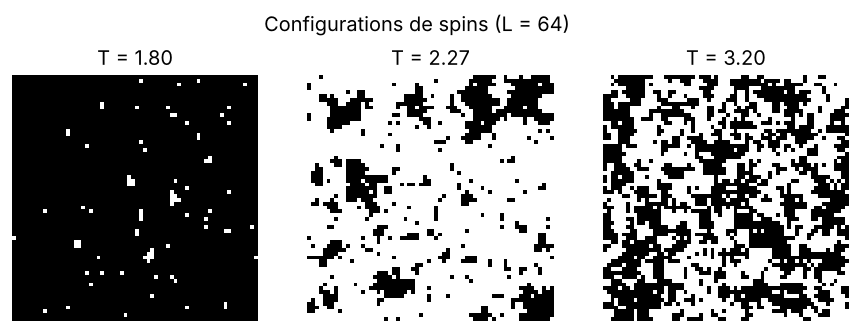
\includegraphics[width=0.95\linewidth]{02-modele-ising-monte-carlo/figures/03_configurations.png}
\end{center}

\vfill
\noindent\textbf{Code source :} \href{https://github.com/IsmailaDEH/Ismaila}{\color{accent}github.com/IsmailaDEH/Ismaila}\\
\textbf{Outils :} Python · NumPy · SciPy · Matplotlib · pytest · GitHub Actions · \LaTeX

\newpage
% ------------------------------------------------------------------ Sommaire / méthode
\section*{Vue d'ensemble}
\begin{tabularx}{\linewidth}{@{}l X l@{}}
\toprule
\textbf{Projet} & \textbf{Domaine} & \textbf{Résultat clé}\\
\midrule
Pendule double & Mécanique non linéaire, chaos & $\lambda = 0{,}75~\mathrm{s^{-1}}$\\
Modèle d'Ising 2D & Physique statistique & $T_c = 2{,}249$ (exact $2{,}269$)\\
Équation de la chaleur & EDP, analyse numérique & ordre $2{,}01$\\
SINDy & Physique + apprentissage automatique & $0{,}13\,\%$ d'erreur\\
Orbites & Mécanique céleste & $T \propto a^{1{,}5000}$\\
\bottomrule
\end{tabularx}

\subsection*{Méthode commune}
\begin{enumerate}
  \item \textbf{Partir de la physique} : équations écrites et expliquées avant le code.
  \item \textbf{Coder les algorithmes soi-même} (RK4, Metropolis, Verlet, régression creuse) pour en maîtriser les erreurs.
  \item \textbf{Valider contre une solution exacte} (Onsager, Kepler, solution analytique) avant d'interpréter.
  \item \textbf{Mesurer} : ordres de convergence, erreurs relatives, tableaux chiffrés.
  \item \textbf{Reproductible} : une commande régénère figures et résultats ; tests automatiques sur GitHub Actions.
\end{enumerate}

% ------------------------------------------------------------------ Projet 1
\section{Pendule double : mesurer le chaos}
\lien{01-pendule-double-chaos}

\noindent Le pendule double est le plus simple des systèmes chaotiques. Les équations de Lagrange sont intégrées avec un schéma Runge--Kutta d'ordre~4 écrit à la main, validé par la conservation de l'énergie et par la période analytique du mode en phase, $T = 2\pi/\sqrt{(2-\sqrt2)\,g/\ell}$. Le chaos est mesuré par l'exposant de Lyapunov maximal (méthode de Benettin) :
\[ \lambda = \lim_{t\to\infty}\frac{1}{t}\ln\frac{\|\delta X(t)\|}{\|\delta X(0)\|}. \]

\begin{minipage}[c]{0.48\linewidth}
\centering\small
\begin{tabular}{@{}lc@{}}
\toprule
$(\theta_1,\theta_2)$ initiaux & $\lambda~(\mathrm{s^{-1}})$\\
\midrule
$(10^\circ, 10^\circ)$ & 0,031\\
$(60^\circ, 60^\circ)$ & 0,057\\
$(120^\circ, -10^\circ)$ & \textbf{0,747}\\
\bottomrule
\end{tabular}\\[8pt]
\begin{tabular}{@{}lc@{}}
\toprule
$\Delta t$ (s) & $\max|\Delta E/E_0|$\\
\midrule
$10^{-2}$ & $8{,}1\times10^{-3}$\\
$5\times10^{-3}$ & $3{,}0\times10^{-4}$\\
$10^{-3}$ & $1{,}9\times10^{-7}$\\
\bottomrule
\end{tabular}
\end{minipage}\hfill
\begin{minipage}[c]{0.48\linewidth}
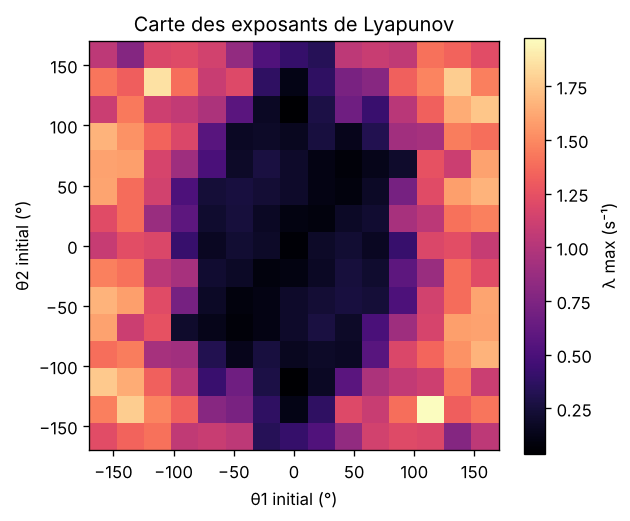
\includegraphics[width=\linewidth]{01-pendule-double-chaos/figures/04_carte_lyapunov.png}
\end{minipage}

\medskip\noindent\textbf{À retenir :} 63\,\% des conditions initiales testées sont chaotiques ; un écart de $10^{-9}$~rad devient macroscopique en moins de 30~s.

% ------------------------------------------------------------------ Projet 2
\section{Modèle d'Ising 2D par Monte-Carlo}
\lien{02-modele-ising-monte-carlo}

\noindent Hamiltonien $H = -J\sum_{\langle ij\rangle} s_i s_j$ sur un réseau carré périodique. L'algorithme de Metropolis est vectorisé par une mise à jour en damier. Le pic de la susceptibilité $\chi = N\beta(\langle m^2\rangle - \langle |m|\rangle^2)$ donne $T_c(L)$, extrapolé par l'analyse de taille finie $T_c(L) = T_c(\infty) + a/L$.

\begin{center}\small
\begin{tabular}{@{}lccc|cc@{}}
\toprule
$L$ & 8 & 16 & 32 & $L\to\infty$ & Onsager\\
\midrule
$T_c(L)$ & 2,512 & 2,402 & 2,304 & \textbf{2,249} & 2,269\\
\bottomrule
\end{tabular}
\end{center}
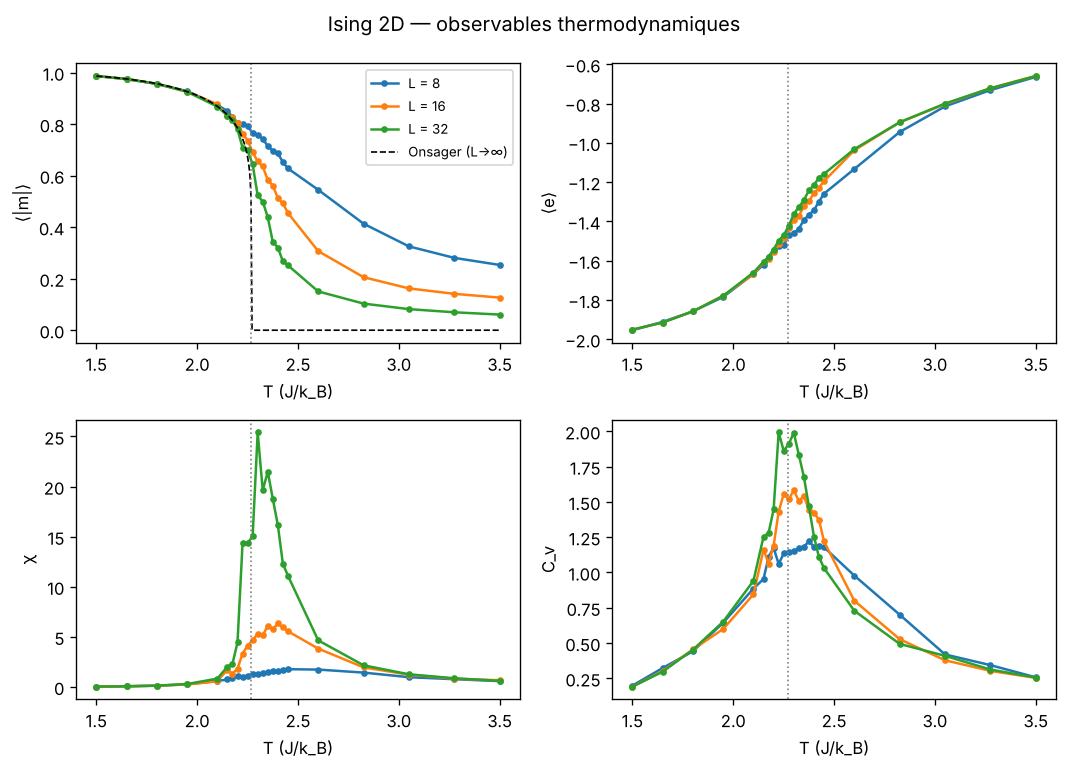
\includegraphics[width=\linewidth]{02-modele-ising-monte-carlo/figures/01_observables.png}

% ------------------------------------------------------------------ Projet 3
\section{Équation de la chaleur : différences finies et stabilité}
\lien{03-equation-chaleur-differences-finies}

\noindent Résolution de $\partial_t u = \alpha\,\Delta u$ par le schéma explicite FTCS en 2D et par Crank--Nicolson en 1D. La solution exacte $u = \sin(\pi x)\sin(\pi y)\,e^{-2\pi^2\alpha t}$ sert de référence.

\begin{center}\small
\begin{tabular}{@{}lcc@{}}
\toprule
Propriété & Théorie & Mesuré\\
\midrule
Ordre spatial FTCS & 2 & \textbf{2,01}\\
Ordre temporel Crank--Nicolson & 2 & \textbf{2,01}\\
Stabilité FTCS 2D & $r = \alpha\Delta t/h^2 \le 1/4$ & stable à 0,25 ; instable à 0,26\\
\bottomrule
\end{tabular}
\end{center}
\begin{center}
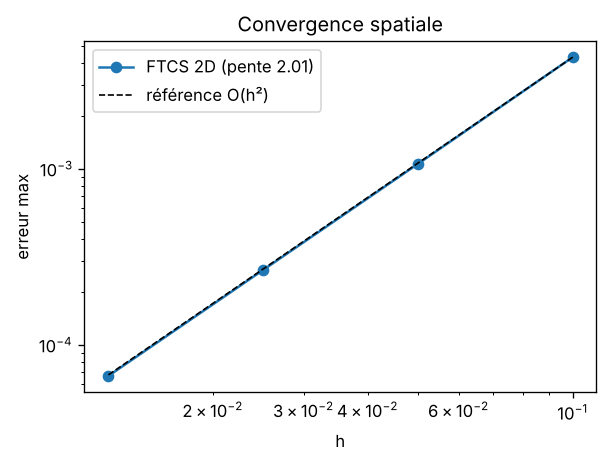
\includegraphics[width=0.48\linewidth]{03-equation-chaleur-differences-finies/figures/01_convergence.png}
\end{center}
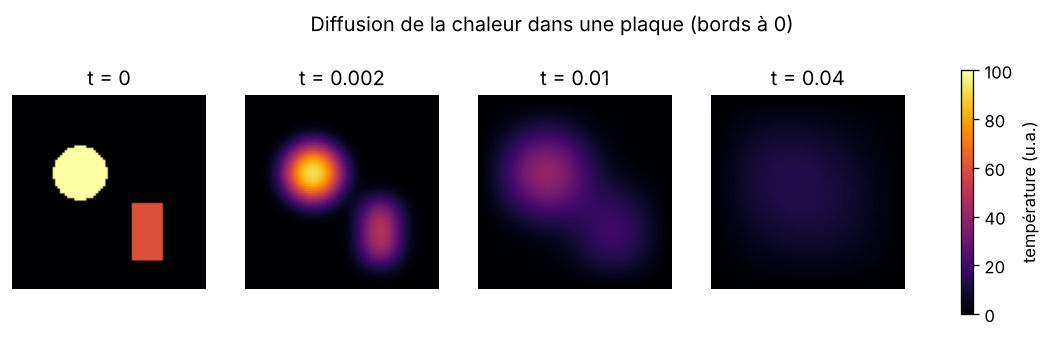
\includegraphics[width=\linewidth]{03-equation-chaleur-differences-finies/figures/02_diffusion_plaque.png}

% ------------------------------------------------------------------ Projet 4
\section{Découverte automatique d'équations (SINDy)}
\lien{04-decouverte-equations-sindy}

\noindent On cherche $\dot X \approx \Theta(X)\,\Xi$ avec $\Theta$ une bibliothèque de monômes et $\Xi$ creuse (régression STLSQ codée de zéro). Les dérivées des données bruitées sont estimées par un filtre de Savitzky--Golay. Test sur le système de Lorenz ($\sigma = 10$, $\rho = 28$, $\beta = 8/3$).

\begin{center}\small
\begin{tabular}{@{}lccccc@{}}
\toprule
Bruit & $\sigma$ & $\rho$ & $\beta$ & Erreur max. & Structure exacte\\
\midrule
0\,\% & 9,999 & 27,992 & 2,666 & 0,03\,\% & oui\\
0,1\,\% & 10,000 & 27,995 & 2,667 & 0,02\,\% & oui\\
1\,\% & 9,994 & 27,963 & 2,666 & \textbf{0,13\,\%} & oui\\
5\,\% & 9,830 & 25,285 & 2,661 & 9,7\,\% & non\\
\bottomrule
\end{tabular}
\end{center}
Équations découvertes avec 1\,\% de bruit :
\[
\dot x = -9{,}99\,x + 9{,}99\,y,\qquad
\dot y = 27{,}96\,x - 0{,}98\,y - 1{,}00\,xz,\qquad
\dot z = -2{,}67\,z + 1{,}00\,xy.
\]
\centerline{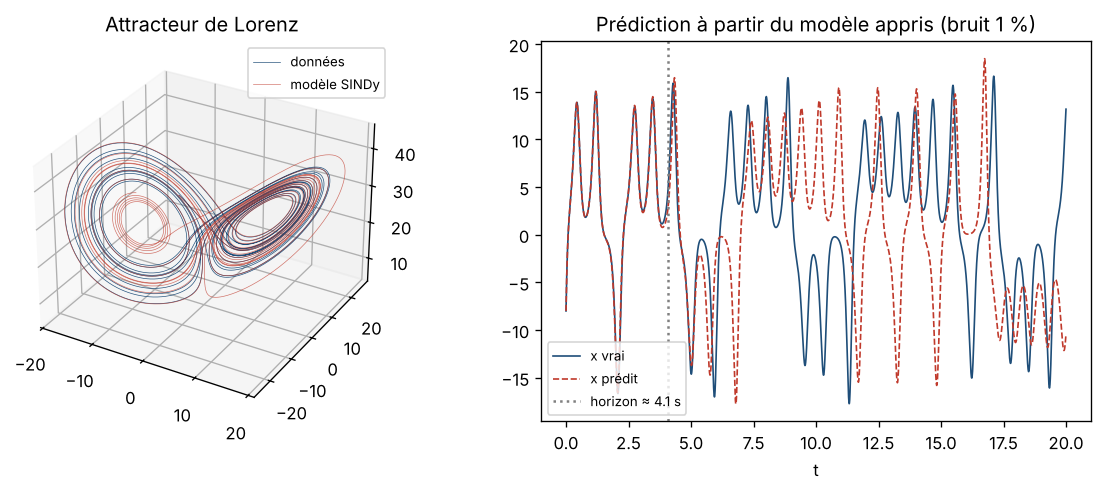
\includegraphics[width=0.85\linewidth]{04-decouverte-equations-sindy/figures/01_attracteur_prediction.png}}

% ------------------------------------------------------------------ Projet 5
\section{Orbites planétaires et intégrateurs numériques}
\lien{05-orbites-kepler-integrateurs}

\noindent Comparaison d'Euler, RK4 et Verlet-vitesse sur une orbite d'excentricité $e = 0{,}6$ pendant 50 révolutions, en unités astronomiques ($GM_\odot = 4\pi^2$).

\begin{center}\small
\begin{tabular}{@{}lcccc@{}}
\toprule
Intégrateur & $|\Delta E/E_0|$ final & $|\Delta L/L_0|$ final & Forces / pas & Comportement\\
\midrule
Euler & 1,1 & $4{,}1\times10^{-1}$ & 1 & la planète s'échappe\\
RK4 & $3{,}3\times10^{-4}$ & $3{,}7\times10^{-5}$ & 4 & dérive croissante\\
Verlet & $\le 7\times10^{-3}$ & $8{,}1\times10^{-15}$ & 1 & erreur bornée (symplectique)\\
\bottomrule
\end{tabular}
\end{center}
\centerline{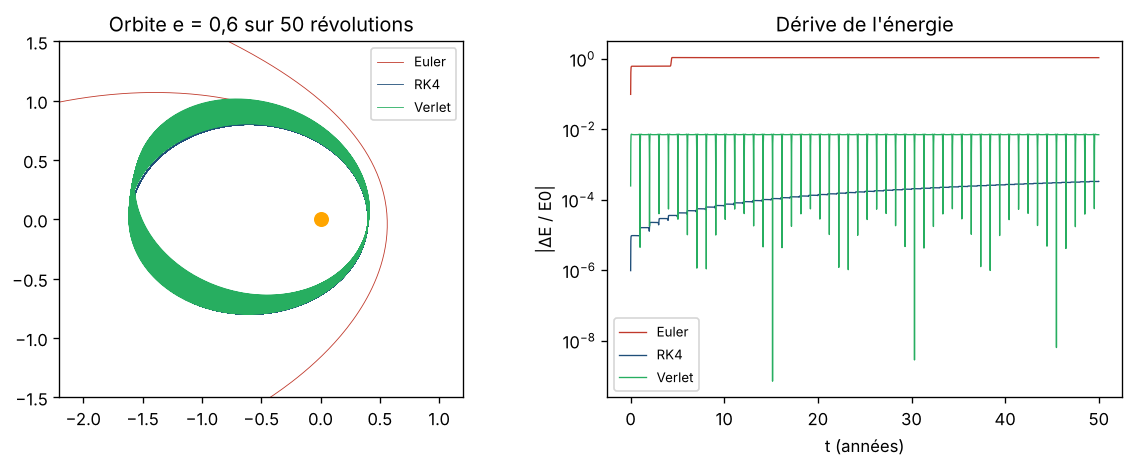
\includegraphics[width=0.8\linewidth]{05-orbites-kepler-integrateurs/figures/01_integrateurs.png}}

\noindent\begin{minipage}[c]{0.55\linewidth}
La 3\textsuperscript{e} loi de Kepler est retrouvée sur six planètes (Mercure à Saturne) : l'ajustement $\log T$ en fonction de $\log a$ donne une pente de \textbf{1,5000} (théorie : $3/2$).
\end{minipage}\hfill
\begin{minipage}[c]{0.40\linewidth}
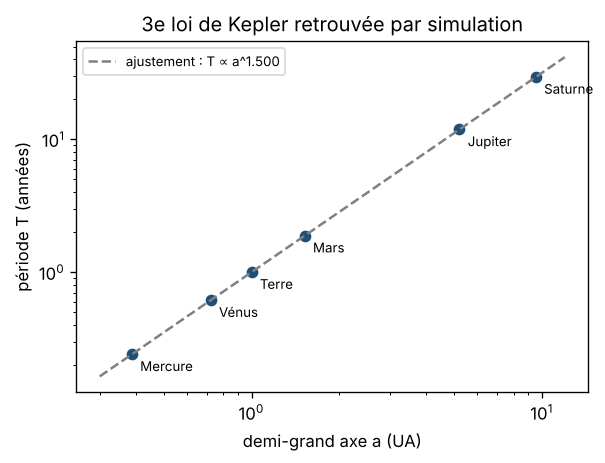
\includegraphics[width=\linewidth]{05-orbites-kepler-integrateurs/figures/03_kepler.png}
\end{minipage}

\end{document}
